\documentclass[english]{sig-alternate}
\usepackage{color}
\usepackage{xcolor}
\usepackage{colortbl}
\usepackage{amstext}
\usepackage{pdfpages}
\usepackage{alltt}
\usepackage{epstopdf}
\usepackage{listings}
\usepackage{xspace,colortbl}
\usepackage[USenglish]{babel}
\usepackage{multirow}
\usepackage{url}
\usepackage{subfigure}
\usepackage{graphicx}
\usepackage{amssymb}
\usepackage{fmtcount}
\usepackage{amsfonts}
\usepackage{xspace}
\usepackage{amsmath}
\usepackage{multirow}
\usepackage[mathscr]{eucal}
%\usepackage{psfrag}
\usepackage{colortbl}
\usepackage{bm}
\usepackage[nospace]{cite}
\makeatletter
\newif\if@restonecol
\makeatother
\let\algorithm\relax
\let\endalgorithm\relax
\usepackage[lined,boxed,vlined,ruled]{algorithm2e}
\special{papersize=8.5in,11in}



\setcounter{secnumdepth}{3}

\long\def\comment#1{}
%\usepackage[dvipdfm]{hyperref}
%\usepackage[dvips]{hyperref}
\begin{document}
%\conferenceinfo{SIGMOD'14,} {June 22--27, 2014, Snowbird, Utah, USA.}
%\CopyrightYear{2014}
%\clubpenalty=10000
%\widowpenalty = 10000

%\hyphenpenalty=5000
\tolerance=1000
\linespread{1}%
%\pagenumbering{arabic}

\title{Deep Clearning: Declarative Big Data Cleaning} 


\iffalse
\author{\alignauthor Sanjay Krishnan,~~Jiannan Wang,~~Sameer Agarwal,~~Michael J. Franklin,~~Ken Goldberg \\
\vspace{.2em}\affaddr{AMPLab, UC Berkeley} \\
\fontsize{9}{10}\selectfont\ttfamily\upshape
\vspace{.1em}\{sanjay,jnwang\}@eecs.berkeley.edu, \{sameerag,franklin\}@cs.berkeley.edu, goldberg@berkeley.edu
}
\fi


%Identifying Similarity Functions from Examples for Effective Record Matching

%\subtitle{[Extended Abstract]
%\titlenote{A full version of this p aper is available as
%\textit{Author's Guide to Preparing ACM SIG Proceedings Using
%\LaTeX$2_\epsilon$\ and BibTeX} at
%\texttt{www.acm.org/eaddress.htm}}}
%\pagenumbering{arabic}

\newtheorem{theorem}{Theorem}
\newtheorem{example}{Example}
\newtheorem{definition}{Definition}
\newtheorem{proposition}{Proposition}
\newtheorem{lemma}{Lemma}
\newtheorem{corollary}{Corollary}
\newtheorem{demonstration}{Demonstration}

\newcommand{\dataset}{data set\xspace}
\newcommand{\datasets}{data sets\xspace}
\newcommand{\biascorrected}{NormalizedSC\xspace}
\newcommand{\bias}{\biascorrected}
%\newcommand{\sampledirty}{\texttt{SampleDirty}\xspace}
%\newcommand{\sampleclean}{\texttt{SampleClean}\xspace}
%\newcommand{\allclean}{\texttt{AllClean}\xspace}
%\newcommand{\alldirty}{\texttt{AllDirty}\xspace}
\newcommand{\sampledirty}{{SampleDirty}\xspace}
\newcommand{\sampleclean}{{RawSC}\xspace}
\newcommand{\allclean}{{AllClean}\xspace}
\newcommand{\alldirty}{{AllDirty}\xspace}
\newcommand{\sys}{\textsf{DeepClearner}\xspace}
\newcommand{\projx}{\sys}
\newcommand{\saqp}{SAQP\xspace}
\newcommand{\saqpplus}{\projx}
\newcommand{\blinkdb}{BlinkDB\xspace}
\newcommand{\ctable}{\ensuremath{T^{clean}}\xspace}
\newcommand{\var}{\ensuremath{\texttt{var}}\xspace}

\newcommand{\attr}[1]{\texttt{#1}\xspace}
\newcommand{\afunc}[1]{\texttt{#1}\xspace}
\newcommand{\M}{\ensuremath{M}\xspace}
\newcommand{\Pset}{\ensuremath{P}\xspace}
\newcommand{\gfunc}{\ensuremath{f}\xspace}
\newcommand{\avgfunc}{\ensuremath{\texttt{avg} }\xspace}
\newcommand{\varfunc}{\ensuremath{\texttt{var} }\xspace}
\newcommand{\productfunc}{\ensuremath{\texttt{product} }\xspace}
\newcommand{\geomeanfunc}{\ensuremath{\texttt{geomean} }\xspace}
\newcommand{\countfunc}{\ensuremath{\texttt{count} }\xspace}
\newcommand{\sumfunc}{\ensuremath{\texttt{sum} }\xspace}
\newcommand{\groupby}{\ensuremath{\texttt{group-by}}\xspace}
\newcommand{\PCset}{\ensuremath{P^{(c)}}\xspace}
\newcommand{\PCseti}[1]{\ensuremath{P^{(c)}_{#1}}\xspace}
\newcommand{\SCset}{\ensuremath{S}\xspace}
\newcommand{\Sset}{\ensuremath{S}\xspace}
\newcommand{\Pseti}[1]{\ensuremath{P_{#1}}\xspace}
\newcommand{\Sseti}[1]{\ensuremath{S_{#1}}\xspace}
\newcommand{\di}[1]{\ensuremath{d_{#1}}\xspace}

\newcommand{\Correct}[1]{\texttt{Correct}\ensuremath(#1)\xspace}
\newcommand{\Remove}[2]{\texttt{Remove}\ensuremath(#1, #2)\xspace}
\newcommand{\Predicate}[1]{\texttt{Predicate}\ensuremath(#1)\xspace}
\newcommand{\Dedup}[2]{\texttt{Dedup}\ensuremath(#1)\xspace}


\def\indistHIGH{\,{\buildrel d \over \rightarrow}\,} 

\newcommand{\reminder}[1] {{{\bf [[[#1]]]}\xspace}}
%\newcommand{\reminder}[1] {}


\newcommand{\ewu}[1]{\noindent{\color{blue}{EWu: #1}}}
\newcommand{\sanjay}[1]{\noindent{\color{red}{SanJ: #1}}}
\newcommand{\haas}[1]{\noindent{\color{red}{Haas: #1}}}
\newcommand{\team}[1]{\noindent{\color{red}{Haas or SanJ: #1}}}
\newcommand{\jn}[1]{\noindent{\color{red}{JW: #1}}}


\pagestyle{plain}





\maketitle
\thispagestyle{plain}



% A category with the (minimum) three required fields
%\category{H.4}{Information Systems Applications}{Miscellaneous}
%A category including the fourth, optional field follows...
%\category{D.2.8}{Software Engineering}{Metrics}[complexity measures, performance measures]
%\terms{Delphi theory}
%\keywords{ACM proceedings, \LaTeX, text tagging}

% !TEX root = demo.tex
\begin{abstract}
Dealing with dirty data is a fundamental barrier in modern data-driven applications -- 
blindly using results that are derived from dirty data can lead to hidden, yet significant, errors.
To combat dirty data, analysts can easily spend 80\% or more of their analysis 
time~\cite{kandel2012} attempting to identify and understand the data errors, 
while concurrently building custom scripts or large data cleaning workflows 
in order to manage and fix the errors.  Because data cleaning is domain-specific and challenging,
designing such workflows is an iterative process that requires a tight interactive feedback loop.

Existing data cleaning systems are either batch-oriented processing
systems that lack interactivity, or interactive systems that are
designed for a specific data cleaning task (e.g., deduplicating
product data, or finding outliers).  In contrast,
we present \sys, a data cleaning system that distills the core components of existing data cleaning
frameworks into a small set of logical operators that can be composed
into data cleaning plans and incorporates techniques that minimize the latency of the feedback
loop and support dynamic reconfiguration while cleaning plans execute.
We overview the system architecture and these techniques, 
then propose a demonstration designed to showcase how \sys can improve iterative data analysis
and cleaning. The code is available at: \url{http://www.sampleclean.org}.
\end{abstract}


% !TEX root = demo.tex
\section{Introduction}\label{sec:intro}

\begin{figure}[t]
\centering
\vspace{-0.5cm}
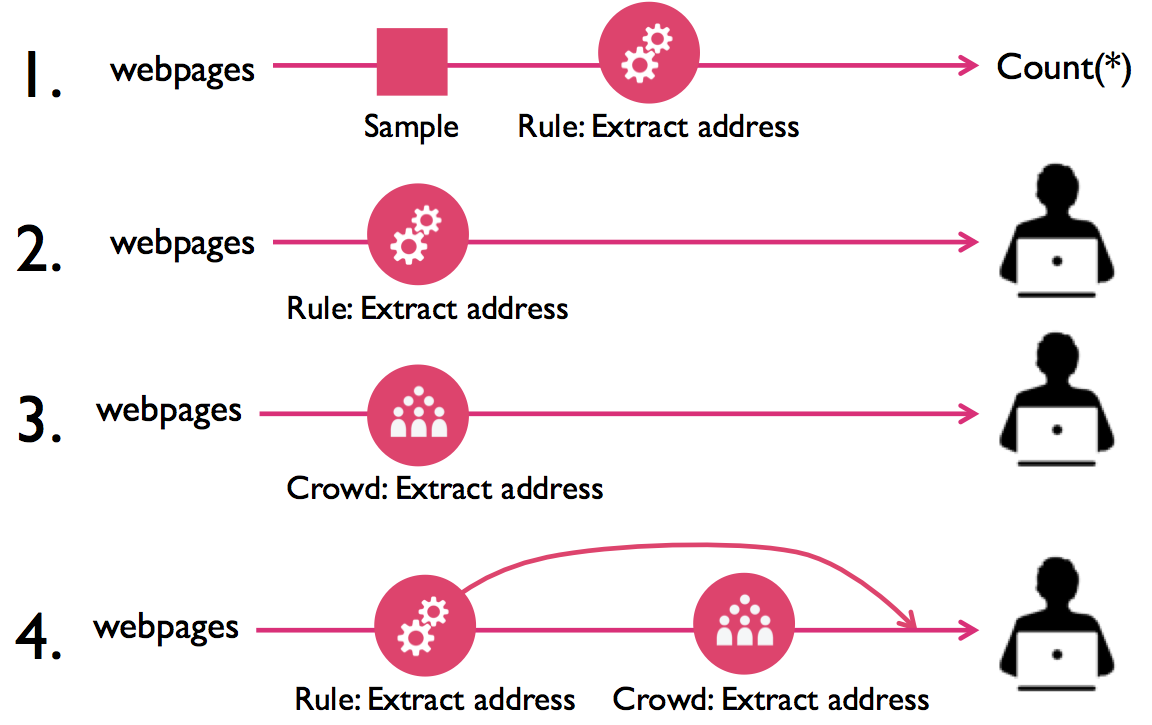
\includegraphics[width = .4\textwidth]{figs/lifecycle.png}
\vspace{-0.2cm}
\caption{Example iterations of the extraction portion of a cleaning pipeline that extracts restaurant information from webpages.  1) User uses a sample to decide if there are enough unique restaurants in the webpages to be worth cleaning.
2) User then runs the rule-based extractor on the whole dataset and inspects the live results.  2) The quality was low, so user moves to a manual human-based solution.  3) The quality is high, but the crowd-based extractor is 
slow. There are enough high quality extractions to train a classifier that decides if the output of the automated process should be sent to the crowd.}
\label{fig:ex-plan}
\end{figure}
% why feedback loops exist/are important (cite Joe’s shit in the past 3 years, blinkdb, etc.). highlight domain specificity. Large variety of data cleaning tasks

%
% Genereal comment that data cleaning is important:
%
The prevalence of dirty data presents a fundamental obstacle to modern data-driven applications, since 
blindly using results that are derived from dirty data can lead to hidden, yet significant errors.
Analysts report spending upwards of 80\% of their time on problems in data cleaning \cite{kandel2012} including 
error diagnosis, instance-specific cleaning scripts, and managing large data ingest pipelines.
The underlying problem is that data cleaning is often specific to the domain, dataset, and eventual analysis,
leading to a breadth of possible errors that are manifest in the data and a variety of options to clean it.
The user must go through the cleaning process with little or no guidance, deciding for each of her data sources what to extract, how to clean it,
and whether that cleaning will significantly change results. 
Without a general, user-efficient, and scalable data cleaning system, analysts have to repeatedly manually construct data cleaning workflows while simultaneously managing a very complex tradeoff space.

Figure~\ref{fig:ex-plan} shows a data cleaning workflow that prepares a dataset of unstructured restaurant webpages for analysis.
In order to run queries over the restaurants, the data analyst must extract structured fields of interest (e.g. address, cuisine category), then eliminate other sources of error, such as duplicate restaurant entries or non-canonical cuisine categories (e.g., `Chinese' vs. `Chinese food'). 
Though these data cleaning requirements have been specified at a logical level, there is a huge space of possible \textit{physical} implementations of the logical operators. 
For example, extraction could be rule-based, rely on structured learning, ask crowd workers to extract the desired data fields, or some combination of all three.
Even after selecting (say) a crowd-based operator, many parameters might influence the quality of the output data or the speed and cost of cleaning it: the number of crowd workers who vote on the extraction for a given webpage, the amount each worker is paid, etc.
A priori, a data analyst has little intuition for what physical plan will be optimal in this large space. 
In practice, she will likely pick a simple default for each logical operator (say, a rule-based extraction), then run data through the workflow and iterate by changing parameters or choosing new physical operators until she is satisfied with the cleaned data.

%The prevalance of data cleaning systems in both the research and industrial communities --
%Corleone does blah, XXX addresses blah. Nadeef does blah -- speak to the importance of a
%data cleaning framework as part of the modern big data ecosystems. \ewu{include open access of data in argument?} \jn{We also need to take a look at data cleaning systems in industry. }


% why existing systems suck aka related work
% 1. have slow feedback loops (dataset-dependence, …)
% 2. solve very specific data-cleaning tasks
Since the beginning of data management, systems have been explored by both the research and industrial communities to improve data cleaning efficiency and quality.
However, no existing systems address the end-to-end data cleaning process described above.
Extract-transform-load (ETL) systems~\cite{informatica,talend,apachefalcon} require developers to manually write data cleaning rules and execute them as long batch jobs, 
and constraint-driven tools that allow analysts to define ``data quality rules" and automatically propose corrections to maximally satisfy these rules \cite{DBLP:conf/sigmod/DallachiesaEEEIOT13}.
Unfortunately, neither provide the opportunity for iteration or user feedback, inhibiting the user's ability to rapidly prototype different data cleaning solutions.
Projects such as Wrangler~\cite{wrangler,trifacta} and OpenRefine~\cite{openrefine} support iteration with user-centric spreadsheet-style interfaces that enable the user to inspect a sample of the dataset, compose data cleaning sequences using a direct manipulation interface, and apply these sequences to the full dataset.
However, they are limited to specific extraction-based cleaning tasks, do not support crowd or machine learning-based refinement at scale, and cannot incorporate user feedback to optimize the data cleaning sequences.
Crowd-based~\cite{gokhale2014corleone,stonebraker2013data} systems have been proposed to relieve the data cleaning analyst of the burden of rule specification or manual cleaning, but are usually very task specific (e.g., de-duplication~\cite{gokhale2014corleone,park2014crowdfill,eracer,chen2014integrating}) and require analysts to awkwardly chain systems together to execute the entire cleaning workflow, preventing end-to-end optimization of the entire plan.
These existing limitations suggest the need for a system that is general enough to adapt to a wide range of data cleaning applications, scales to large datasets, and natively supports fast-feedback interactions to enable rapid data cleaning iteration.

In this paper, we introduce \sys, a system designed to support such a workflow end to end.
\sys allows users to specify declarative data cleaning plans composed of rule-based, learning-based, or crowd-based operators, then makes cost-aware recommendations for improving the accuracy or latency of a plan by swapping in new physical operators or modifying their parameters.
\sys supports rapid iteration on plans by providing users with the opportunity to provide ground-truth feedback after each logical operator in the plan, improving recommendations, and provides efficient support for making adjustments to in-flight plans using caching and tuple lineage.

Supporting these capabilities requires a mixture of careful engineering 
as well as tackling several research challenges:

\squishlist
\item {\bf Operator and API design}: We have designed a core set of logical data cleaning operators --
filter, similarity join, extract and sample -- that can be composed to
implement high-level cleaning tasks such as entity resolution.  Operators support
rule-based, learning-based, and crowd-based physical implementations. 
To support crowd-based cleaning operators, we have developed a crowd-managment 
framework that delivers data cleaning tasks to multiple crowdsourcing platforms using a common API.

\item {\bf Near-instant feedback}: We accelerate feedback loops in the system with techniques to reduce both 
intra- and inter-operator latencies. To improve Crowd operator performance, we leverage techniques such as straggler 
mitigation~\cite{venkataraman2014power}, worker latency modeling, and bandit algorithms~\cite{thompson1933likelihood}
to consistently retrieve crowd results in seconds rather than hours. To reduce latencies at a plan level, we allow data cleaning to 
proceed asynchronously and allow users to introspect and modify data cleaning plans at any point during their execution.

\item {\bf Hot Swapping}: In contrast to batch-oriented data cleaning, rapid iteration necessitates the
ability to tune an operator parameter or reconfigure the sequence of cleaning operators as the cleaning
plan is running.  We develop techniques that leverage tuple lineage to intelligently cache intermediate results to minimize
re-computation when an in-flight plan has been modified.
\squishend


In our demonstration, we will run an entity resolution plan on two restaurant datasets, and
show how \sys can be used to 1) specify and execute a data cleaning plan using our domain specific
language, 2) quickly clean a sample to characterize how a plan is performing, 
3) observe that cleaning plans are not necessarily optimal across datasets, and 
4) incrementally refine the plan to fit a new dataset by changing an operator's parameter (e.g., similarity threshold)
or its physical implementation.
The fourth interaction lets the participants inspect the effects of different physical plans.
Users can then execute a plan over a live crowd that uses the audience as workers, or a simulated crowd
that uses pre-collected crowd responses. The dashboard (Figure~\ref{screenshot-rec}) also provides a live inspection
interface to view the status of the cleaning plan as it executes.



%Our contributions/requirements
%different ways to tighten the feedback loop:
%end-to-end latency/cost (operator optimization)
%looking versus touching
%Adding introspection (more points of observation)
%hot-swapping (more points of changing plans)
%We have built an end-to-end data cleaning framework with these requirements in mind. (... things we do …) (... engineering contributions …).
%In this demonstration, we highlight the benefits of improving feedback loops for data cleaning using X datasets by optimizing a data cleaning pipeline for one data set/cleaning task, then quickly fitting the pipeline to another dataset.


\if{0}

\jn{Honestly, I didn't quite buy declarativity of the system. In my opinion, data cleaning is so domain specific. It's hard to make it declarative. For a given domain, people may need to write their own data cleaning system. There is a lack of a data cleaning framework that they can build based on. This motivates us to develop such framework. 


We analyze a large variety of domain specific data cleaning systems, and identify several key components: declarative data cleaning operators (e.g., similarity joins), active learning, and crowd/expert sourcing platforms that they require. In our framework, we abstract these components, and implement them in a general way. 

We mainly address two challenges: extensibility and scalability. For the former one, we came up with a nice data-cleaning pipeline API, which people can easily use to compose their own data cleaning tasks. For the latter one, we address it in two aspects: Sampling + Asynchrony.}

\ewu{That's fair, will need to address why a framework is necessary and what benefits it provides.  I think a framework is the correct pitch, hard to sell a set of operators.  Are the above challenges -- extensibility and scalability -- actually difficult?  Worried it's straightforward application of existing techniques.}



In contrast, our work is based on the observation that the majority of data cleaning workflows
can be decomposed into a small set of logical operations (in addition to traditional database operators):
filter based on constraints, extract new fields from existing data, and a similarity join to match
similar or duplicate records. \ewu{quickly validate why this observation holds.} \jn{Yes! I also found that Sec 2.3 has more operators than you describe here.}  
By designing a system around these core operators, we can provide a vast library of physical  
data cleaning operators that span the range of algorithmic, machine learning, and human computation-based
implementations that are necessary practical data cleaning pipelines.   \ewu{Describe live inspection as 
a core feature or is it too easy?}

Designing such a system requires tackling several design challenges:

\begin{enumerate}
\item Speed
\item Quality
\item API Design/extensibilty
\end{enumerate}



We have implemented an initial version of \sys on top of the AMPLab Spark stack, which provides us 
with access to its advanced distributed processing and machine learning features.  Our goal for the current
version is to implement the core mechanisms for declarative specification of the
data cleaning pipeline, solidify the API design, and incle support for, and implementations of,
multiple classes of physical data cleaning operators.


\fi



\if{0}

Cleaning, pre-processing, and formatting data is a required first step in any data analytics pipeline.
However, despite this importance, large-scale data analytics platforms such as Spark or Hadoop lack integrated data cleaning frameworks.
There are a few challenges in building a general purpose data cleaning framework: (1) data cleaning is often
domain specific and requires specialized software targeted at one or a handful of data sources \cite{wang1999sample}, (2) data cleaning is often 
expensive as it increasingly involves human effort via crowdsourcing or experts \cite{DBLP:conf/sigmod/GokhaleDDNRSZ14}, and (3) learning how to clean dirty data from examples
is often hard without a greatly restricted set of operators \cite{DBLP:conf/uist/GuoKHH11}.

We address this problem in \projx by designing a Spark library of composable and scalable data cleaning primitives.
\projx abstracts the logical data cleaning operators: Extraction, Similarity Join, Filtering, from the physical implementation i.e, Rule, Crowd, or Machine Learning.
We interface these primitives through a DSL with which a user can build data cleaning operators that suit their needs.
\projx provides transparent optimizations for each of the components and their composition.
In this demonstration proposal, we present \projx and highlight some of its key features.
While there are many existing systems that do one aspect of data cleaning and transformation (e.g Entity Resolution or Extraction), 
many real world data cleaning tasks have multiple types of errors.
Composing disparate systems can lead to complex code and inefficiencies at scale.
With \projx, we hope to design a set of optimized composable primitives that span a large space of data cleaning tasks.

The first key feature of \projx is that it provides optimized distributed implementations 
of the physical data cleaning operators.
For example, a key step in many deduplication algorithms is a Similarity Join which finds all pairs of records that are within some similarity threshold.
A naive implementation of a Similarity Join would apply a similarity function to all pairs of records.
However, in \projx, we provide optimized implementations of certain common similarity functions (e.g Jaccard, Edit Distance, etc.) that allow for 
a combined broadcast join and prefix filtering which intelligently skips pairs of records using a broadcasted inverted index.

Another feature of \projx is managing the latency and the scale problems of crowd-based data cleaning. 
Crowdsourcing is increasingly prevalent in data cleaning, and \projx provides physical crowd-based implementations
of the logical operators.
However, crowds work at a different latency and scale point in comparison to distributed analytics platforms.
To address the latency problem, we build asychrony into the system.
The user can query intermediate results at any time as crowd responses stream in.
To address the scale issue, \projx provides sampling primitives.
The glue that ties all of the crowd components together is a Machine Learning technique called Active Learning.
As we collect more and more crowd responses, we learn a model that predicts these responses to apply it on the uncleaned data.
Active Learning selects the most informative questions to ask the crowd.

Finally, \projx provides an approximate query processing (AQP) framework.
With slow asynchronous data cleaning algorithms as in crowdsourcing, we need 
to define clear semantics for the intermediate results.
Our AQP framework uses the algorithms proposed in \cite{wang1999sample}, to estimate and bound early results.
It is also common for data scientists to prototype expensive data cleaning pipelines on samples and AQP allows quick evaluation of
aggregate query results on a cleaned sample.

\subsection{Demonstration Scenario}
\reminder{TODO}

\fi




\if{0}
Consider for example, the ability to rapidly understand the types of errors that are present, as well as prevalance of 
these errors is cruicial.



Before an organization can use a new dataset as part of their analysis pipeline
(e.g., to build complex learning models or answer analyst queries)
the errors in the dataset need to be removed in order to ensure accurate conclusions.  

Modern data-driven organizations rely on the ability to ingest and generate large data sets from 
disparate sources, and combine the data together to build complex models or answer analytical questions.  
For example, a restaurant review website may collect restaurant listings by scraping data from webpages or purchasing them from external sources, and
restaurant visitation information for sources such as OpenTable or FourSquare, and aggregate the data to
model user eating habits.  
The set of cleaning tasks necessary for each of these data sources is highly domain and application specific,
and oftentimes the developer is concurrently trying to clean the data source as well as understand its properties.


Oftentimes, these data sources have data quality issues that require a complex data cleaning pipeline -- 
e.g., data extraction, re-formatting, identification and fixes of missing or incorrect values,
and removal of redundant information -- before the data is useable by downstream processes.
Data sources are often domain specific and new for the data analyst, 
As datasets continue to grow, and organizations make use of mure and more datasets, the ability to
rapidly clean the data is more important.  
\fi

% !TEX root = demo.tex
\section{System Architecture}

In this section, we provide a brief overview of the \sys system and its APIs.
Figure~\ref{fig:arch} depicts the system architecture.

\begin{figure}[t]
\centering
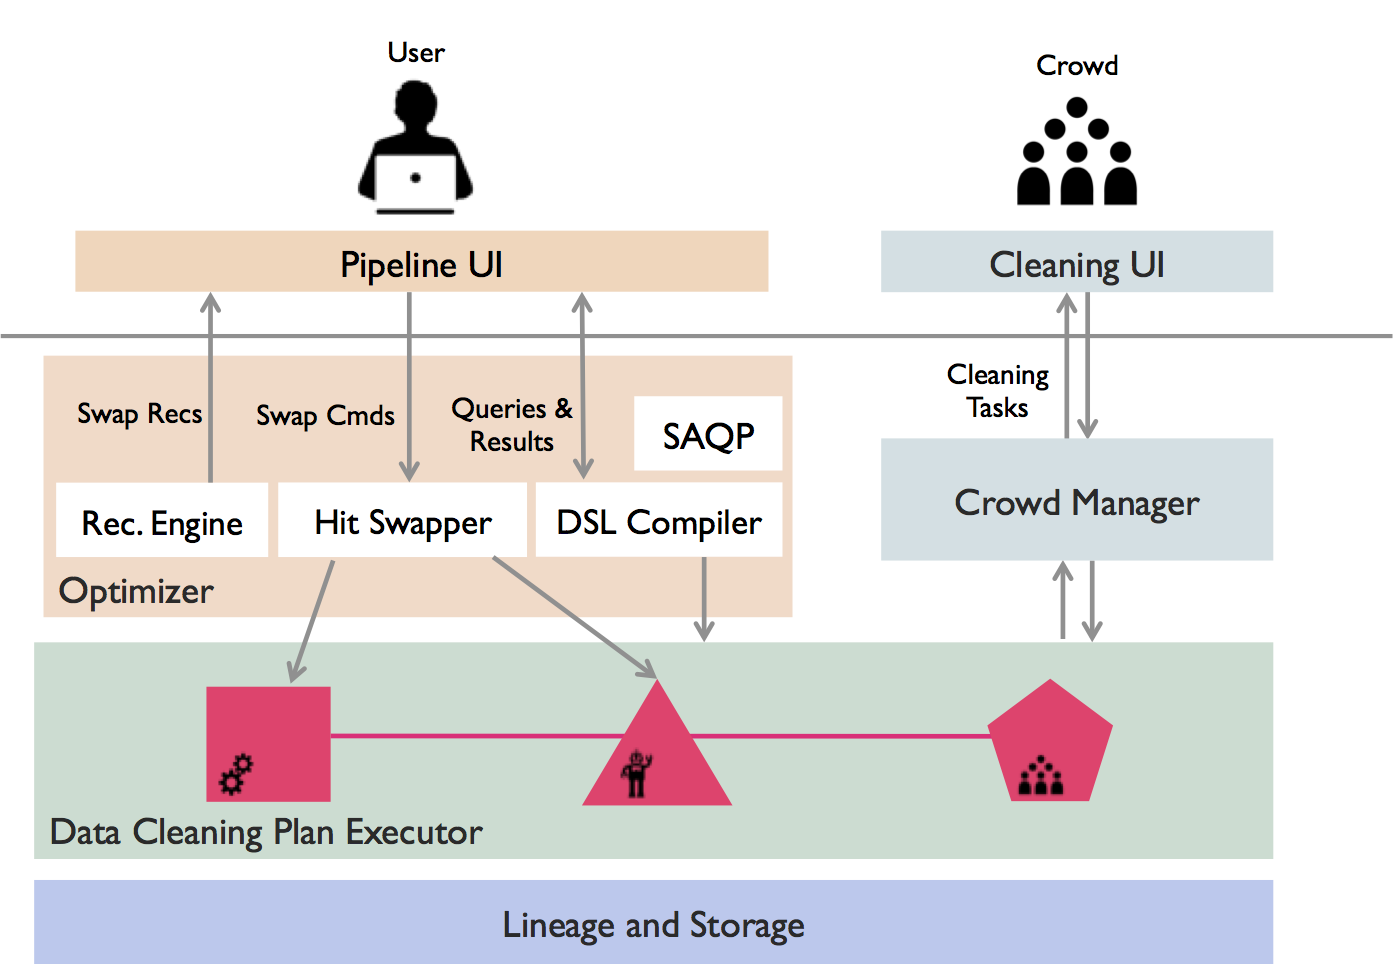
\includegraphics[width = .5\textwidth]{figs/architecture.png}
\caption{\sys system architecture, with an example entity resolution pipeline.}
\label{fig:arch}
\end{figure}

\subsection{Architecture Overview}
The \sys architecture is focused on providing UI, language, and systems tools for building pipelines for data cleaning. 
Users interact with the system through the pipeline UI, which allows them to compose data cleaning workflows from modular operators.
These pipelines are synthesized as expressions in our data cleaning language (section~\ref{sec:dsl}), then compiled into physical cleaning plans.
As data cleaning executes, users can interact with the pipelines via tight feedback loops in two forms.
First, users can issue queries and observe approximate results based on the data that has been cleaned thus far.
Second, users can pick from a set of recommended modifications to their pipeline (for example, making a similarity join more permissive) and modify the data cleaning in-flight by \textit{hot-swapping} components of the pipeline.
Data is stored in a relational engine that tracks pipeline lineage with each tuple in order to enforce the semantics of hot-swapping correctly on in-flight tuples.
Logical cleaning operators may have a number of physical implementations (section~\ref{sec:operators}).
Automated rule-based or learning-based operators leverage Spark and MLLib for efficient distributed computation, and operators that require human intervention call out to \sys's crowd manager API, which renders data cleaning tasks and displays them to crowd workers across multiple crowds (e.g., Amazon Mechanical Turk) for processing.

\subsection{Cleaning DSL}
\label{sec:dsl}
We provide a language for specifying the composition of data cleaning operators.
The logical operators define the input and output behavior of the operation and 
the physical operators specify the implementation.
The general syntax of this language is:
\begin{lstlisting}
<logical operator> on <relations>
	with <physical operators> , <params>
\end{lstlisting}

These expressions are composable:
\begin{lstlisting}
R1 := <logical operator> on <relations> 
	with <physical operators> , <params>
R2 := <logical operator> on R1 
	with <physical operators> , <params>
\end{lstlisting}
\projx provides an integration layer of these expressions with Scala/Apache Spark allowing for the manipulation of SchemaRDDs (Spark RDDs with additional schema information):
\begin{lstlisting}
val rddA = spark.textFile(file).toSchemaRDD
val cleanData = clean(rddA,<expression>)
\end{lstlisting}

\subsection{Cleaning Operators}
\label{sec:operators}
\sys supports a small set of operators that can express a wide variety of common data cleaning workflows. For example, the pipeline depicted in in Figure~\ref{fig:arch} performs crowd-based entity resolution: the similarity join operator generates candidate tuple pairs (the \textit{blocking} step), and the crowd-based filter operator uses humans to identify duplicates from the candidates (the \textit{matching} step). Additional operators include Extraction, Sampling, and Active Learning.

Individual logical operators have multiple physical implementations, each with its own cost, latency, and accuracy profile. For example, crowd-based implementations tend to be high cost, high latency, and high accuracy, whereas rule-based implementations tend to be low cost, low latency, and low accuracy. The \texttt{with} clause of our data cleaning language allows users to explicitly specify desired physical operators, and \sys's recommendation engine provides actionable suggestions for modifying the pipeline to navigate the tradeoff space.






%\subsection{Logical Operators}
\projx specifies three logical operators: Extraction, Filtering, and Similarity Join. 
\sanjay{In depth why these operators are {\it sufficient}.}

For performance (or some other reason), we support several additional
logical operators tha enable optimization: Sampling, Async, and Transitive Closure.
The composition of these operators support a variety of data cleaning
operations. 
For example, a deduplication task can be expressed as a Similarity Join to pair similar records
together and then a filtering task to remove false positives.
These logical operators specify the input and output data schema and allow us to compose operations.


\vspace{0.5em}

\noindent \textsf{SimilarityJoin(R,S,$\phi$, $t$)}: For a given relations $R(a_1,...,a_l)$ and $S(b_1,...,b_k)$, a similarity function $\phi$, and a threshold $t$, the similarity join of R and S is defined by:
\[
\{ (r,s) \in R \times S \text{ s.t } \phi (r,s) \ge t \}
\]

\vspace{0.5em}


\noindent \textsf{Filter(R, $\rho$)}: For a given relation $R(a_1,...,a_l)$ and a boolean condition $\rho$, return $R' \subseteq R$ that satisfies $\rho$.

\vspace{0.5em}

\noindent \textsf{Extract(R, a, $\epsilon$)} For a given relation $R(a_1,...,a_l)$, a attribute $a$, and an extraction function $\epsilon$, apply $\epsilon$ to every $R(a)$ returning $\epsilon(R(a)) = (v_1,...,v_k)$. The result relation is:
\[
R(a_1,...,a_l,\epsilon(R(a)))
\]

\noindent \textsf{Sample(R, $m$)}: For a given relation $R(a_1,...,a_l)$ and return $R' \subseteq R$ such that each $r \in R$ is in $R'$ with probability $m$.

\vspace{0.5em}

\noindent \textsf{Project(R, $p_1,...,p_k$)}: For a given relation $R(a_1,...,a_l)$ and return $R(p_1,...,p_k)$.

\vspace{0.5em}

\noindent \textsf{TransitiveClosure(R,$f$)}: For a given relation of pairs of rows from the same base relation, e.g the result of a self-Similarity Join, $R(a_1,...,a_l, b_1,...,b_l)$ return the transitive closure of the relation $S(a_1,...,a_l)$. $f$ is called a cannonical representation function, this takes a set of associated records and returns a single record that is designated as the canonical representation.






%\section{Physical Operators and Implementation}

For each of the logical operators there are different physical implementations.
We do not currently select the appropriate physical operator and the user has to specify this.
We do, however, set sensible default parameters for each of the physical operators.
In \projx, there are three broad categories of physical operators: Automated, Crowd, and Learning.
An automated physical operator is conceptually the same as a SQL user defined function, while a crowd operator uses a microtask platform.
A learning operator takes in training examples (whether crowd or ground truth) and learns an automated operator.
We describe each below.

\ewu{below are straightforward physical implementations of the
logical operators.  Is there anything interesting to say about their
design or a specific physical operator?}

\team{How do we know when transitive closure/any of the physical operators can be safely applied?  Are there properties of the physical ops that could tell us?}


\subsection{Similarity Join} 
\projx provides a library of the following commonly used similarity functions: \textsf{JaccardSimilarity}, \textsf{DiceSimilarity},
\textsf{CosineSimilarity}, \textsf{OverlapSimilarity}, and \textsf{EditDistance}.
The user can select one of these similarity functions.
A naive implementation of a Similarity Join is to take the cartesian product and then filter all pairs of record of similarity greater than $t$.
However, the implemented similarity functions are all symmetric and the similarity function is maximized when $r = p$.
So it suffices to compute a similarity $\theta$-join instead of the full Cartesian product.
We can further add an optimization called prefix filtering to further reduce the number of similarity function evaluations.
In prefix filtering, we prune pairs that cannot possibly meet the threshold $t$ based on the number of tokens that overlap which can be determined with an inverted index.


\subsection{Extraction}
We implement basic automated extraction libraries including delimited splitting and regular expression methods.
However, extraction is a task that is well suited for crowd sourcing.
We provide a parametrized interface that allows the user to specify an extraction attribute, a formatting question, and request data from the crowd.
In Figure \ref{fig:entry}, we illustrate an example of this task.

\begin{figure}[ht!]
\centering
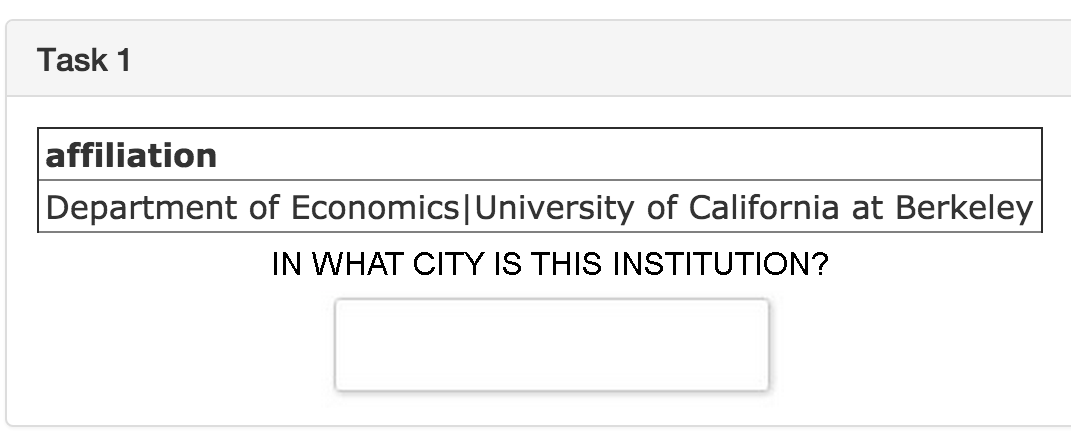
\includegraphics[scale=0.25]{figs/entry.png}
\caption{Example of the Extraction Crowd Interface. \label{fig:entry}}\vspace{-.5em}
\end{figure}

\subsection{Filtering}
We provide an interface for a user defined predicate.
However, as with extraction, filtering has many opportunities for crowdsourcing.
For a filtering operation, the crowd response is binary in contrast to Extraction.
We provide crowd templates for two types of filtering tasks.

\noindent\textbf{Condition Checking: } Given a single record, a crowd worker indicates if it satisfies some condition. In Figure \ref{fig:condition},
we illustrate an example condition checking task.
\begin{figure}[ht!]
\centering
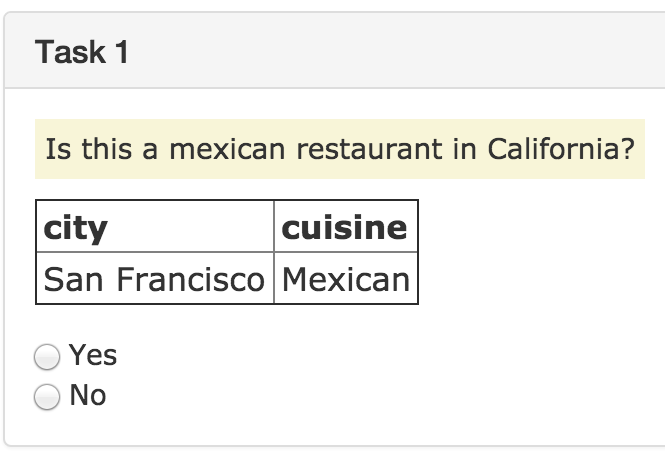
\includegraphics[scale=0.25]{figs/condition.png}
\caption{Condition checking is one variant of the filtering crowd interface.\label{fig:condition}}\vspace{-.5em}
\end{figure}

\noindent\textbf{Pair Comparison: } Given a pair of records, a crowd worker indicates if they are the same or are different. In Figure \ref{fig:pair},
we illustrate an example pair comparison task.

\begin{figure}[ht!]
\centering
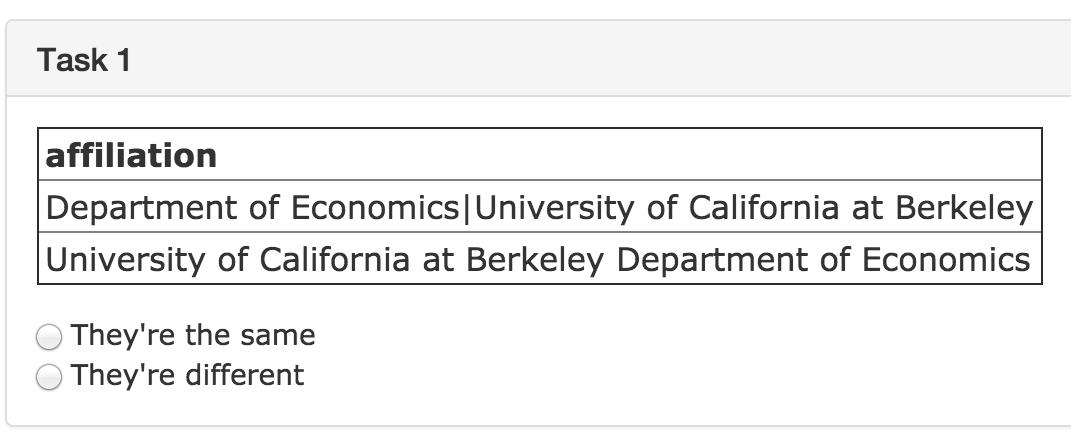
\includegraphics[scale=0.25]{figs/pair.png}
\caption{Pair comparison is the other variant of the filtering crowd interface.\label{fig:pair}}\vspace{-.5em}
\end{figure}



\subsection{Extended Operators}

\subsubsection{Sampling}
\projx provides different variants of uniform sampling.
We provide Bernoulli sampling (in which flips a ``biased coin" for each row) or hash sampling (which hashes an attribute).
Hash sampling allows for joining sampled relations with foreign key relationships.
On the other hand, Bernoulli sampling is less sensitive to skews and leads to more consistent sample sizes.

\subsubsection{Transitive Closure}
Similarity Joins can create issues with transitivity.
For example, rowA might be similar to rowB and rowB might be similar to rowC, but rowA might not be similar to rowC.
We can associate these relationships with edges in a similarity graph.
Then to enforce transitive closure, we solve a connected components problem.
We apply a distributed using a distributed gather-apply-scatter connected components algorithm in the Spark-integrated graph library GraphX.




 %!TEX root = demo.tex
\section{Logical Operators}


\ewu{INSERT: implementation in Spark}

Now, we discuss the logical operators and their parameterization defined in \projx.

\vspace{1em}


\subsection{Research Challenges}

Architecturally, we separate crowd sourcing and automated data cleaning.
There is a crowd server that acts as a layer of indirection between the Spark codebase and crowd sourcing APIs.

\team{Describe Research Challenges.  To what extend can we actually do
optimization given the physical operators?  Unlike relalgebra, the physical operators here are
not interchangable!}



\subsection{Learning Parameters From Example}
In simple cases, it might be easy to use domain knowledge to select and tune physical operators. 
In more complex cases, it might be easier to specify a sample of dirty and clean data instead of the function.
It may also not be feasible to have the crowd clean the entire dataset.
In these cases, we want to learn a statistical model from which we can extrapolate those responses to the rest 
of the data.

In our current implementation of \projx, we pose this learning problem as classification problems.
In general, these parameter functions can be quite complex and this is a simplification of the learning problem.
The choice of classifier and featurization is upto the user. 
We currently support Support Vector Machines and Decision Trees with a featurization library that includes common text processing features.

\vspace{0.5em}

\noindent \textsf{Filter(R, $\mathcal{T}^+$, $\mathcal{T}^-$)}: Given a set of positive training examples $\mathcal{T}^+$ (i.e, $r$ that satisfy the condition) and
negative training examples $\mathcal{T}^-$ (i.e, r that do not satisfy the condition), we learn a classifier that predicts whether a record satisfies the condition. 

\vspace{0.5em}

\noindent \textsf{Extract(R, a, $\mathcal{T}$)} We restrict the learned problem setting to delimited extraction. Given a set of training examples $R(a)$ and the output $v_1,v_2,...,v_k$, we learn a classifier to predict which characters in $R(a)$ are delimiters based on the tokens in the string.

\vspace{1em}

To acquire the samples of clean data, uniform sampling may not be the best strategy.
For example, if there examples of dirty data are very rare, we will not be able to learn a model.
We implement a technique called Active Learning to sample.
Active Learning selects the most informative examples based on the current model so far.
We use an Active Learning algorithm called uncertainty sampling to do this.




\subsection{Inspection}

Data cleaning requires inspection -- user wants to see how the dataset
has been "cleaned"  through the pipeline.  What does that even mean?

\subsection{Dynamic Re-optimization}

Crowd means want to swap in or out operators at run time.


\subsection{Lineage}

\noindent\textbf{Lineage: }
We track the lineage of rows using a primary key.
Users are not allowed to modify this primary key with any operations.
This allows us to apply operations like transitive closure even after projection since we have a unique identifier for each row.

\vspace{0.5em}
\noindent \textbf{Example: } Suppose, we are interested in deduplication of unstructured data. Then, we could apply the following logical operations.
We first apply an \textsf{Extract} operation to extract the unstructured data into columns. If some of the columns are inconsistent in their representation,
we apply \textsf{Project} to those columns that are inconsistent. We can then take a \textsf{SimilarityJoin} to group rows that are similar, and finally
we resolve those differences with \textsf{TransitiveClosure}.



\subsection{Engineering Challenges}
In addition to the numerous research challenges, there have been substantial challenges in engeering \sys.
We highlight two key challenges which are API design and Crowdsourcing.

\subsubsection{API Design}
Many of the research challenges in \sys rely on clear specifications of the input and output behaviors of
the data cleaning operators.
For example, Hot Swapping, is only possible if two physical operators have exactly the same input and output specification.
The engineering challege to to retain modularity and extensibility while restricting operators.
We build a class heirarchy of data cleaning operators which through inheritance and parameterization specify clear input and output behaviors.

One example of this is the Similarity Join operator.
Users might chose complex similarity functions making it hard to understand their semantics for optimization.
We abstract the similarity function into a abstract class called a \textsf{SimilarityFeature}, this class is parameterized
by a single threshold, contains an API to specify whether two records are similar based on the threshold, maintains its
own tokenizer, and has an API to specify available optimization properties such as monotonicity and prefix-filtering.
So if a user proposes an arbitrary similarity function, as long as it is implemented in the API, it can benefit from our
parameter tuning recommendations.

One draw back of an extensive API is that the choices may overwhelm a user.
Many of our API methods and classes come with inherited sensible defaults.
For example, if the user fails to completely specify the semantics of the similarity function through the API, 
the system will avoid optimizations and perform a naive cartesian products and filtering.
These behaviors come naturally through the use of inheritance and polymorphism.

\subsubsection{Crowdsourcing Platform}
The second engineering challenge is designing a platform to serve crowd tasks.
First, working with crowds is inherrently challenging.
Unlike for our automated operators, we have to manage greatly varying crowd worker
response times and quality.
We developed a ``crowd server" to add a layer of indirection to support this.
The crowd server handle serving and processing crowd tasks, including quality control through redudancy.
We aggregate redundant responses using an Expectation-Maximization algorithm.
Only after collecting sufficent confidence for a task, we process that tuple in our pipeline.

The other benefit of a crowd server is that the APIs for Amazon Mechanical Turk (AMT), Crowd Flower, and others greatly vary.
One common feature of these APIs is that they serve tasks through a browser-based interface.
Our crowd server generates tasks in the form of dynamic web pages and process responses through AJAX call backs.
As a result, the same server works for a variety of different crowds including AMT, Crowd Flower, and a custom ``Internal Crowd".
% %!TEX root = demo.tex
\section{Logical Operators}
Now, we discuss the logical operators and their parameterization defined in \projx.

\vspace{0.5em}

\noindent \textsf{SimilarityJoin(R,S,$\phi$, $t$)}: For a given relations $R(a_1,...,a_l)$ and $S(b_1,...,b_k)$, a similarity function $\phi$, and a threshold $t$, the similarity join of R and S is defined by:
\[
\{ (r,s) \in R \times S \text{ s.t } \phi (r,s) \ge t \}
\]

\vspace{0.5em}


\noindent \textsf{Filter(R, $\rho$)}: For a given relation $R(a_1,...,a_l)$ and a boolean condition $\rho$, return $R' \subseteq R$ that satisfies $\rho$.

\vspace{0.5em}

\noindent \textsf{Extract(R, a, $\epsilon$)} For a given relation $R(a_1,...,a_l)$, a attribute $a$, and an extraction function $\epsilon$, apply $\epsilon$ to every $R(a)$ returning $\epsilon(R(a)) = (v_1,...,v_k)$. The result relation is:
\[
R(a_1,...,a_l,\epsilon(R(a)))
\]

\noindent \textsf{Sample(R, $m$)}: For a given relation $R(a_1,...,a_l)$ and return $R' \subseteq R$ such that each $r \in R$ is in $R'$ with probability $m$.

\vspace{0.5em}

\noindent \textsf{Project(R, $p_1,...,p_k$)}: For a given relation $R(a_1,...,a_l)$ and return $R(p_1,...,p_k)$.

\vspace{0.5em}

\noindent \textsf{TransitiveClosure(R,$f$)}: For a given relation of pairs of rows from the same base relation, e.g the result of a self-Similarity Join, $R(a_1,...,a_l, b_1,...,b_l)$ return the transitive closure of the relation $S(a_1,...,a_l)$. $f$ is called a cannonical representation function, this takes a set of associated records and returns a single record that is designated as the cannonical representation.

\vspace{1em}

\noindent\textbf{Lineage: }
We track the lineage of rows using a primary key.
Users are not allowed to modify this primary key with any operations.
This allows us to apply operations like transitive closure even after projection since we have a unique identifier for each row.

\vspace{0.5em}
\noindent \textbf{Example: } Suppose, we are interested in deduplication of unstructured data. Then, we could apply the following logical operations.
We first apply an \textsf{Extract} operation to extract the unstructured data into columns. If some of the columns are inconsistent in their representation,
we apply \textsf{Project} to those columns that are inconsistent. We can then take a \textsf{SimilarityJoin} to group rows that are similar, and finally
we resolve those differences with \textsf{TransitiveClosure}.

\section{Optimized Physical Operators}
Now we discuss the physical implementations of these operators.
There are a variety of optimizations and concerns of each of the operators, in this paper, we 
only highlight the main features.

\subsection{Similarity Join} 
\projx provides a library of the following commonly used similarity functions: \textsf{JaccardSimilarity}, \textsf{DiceSimilarity},
\textsf{CosineSimilarity}, \textsf{OverlapSimilarity}, and \textsf{EditDistance}.
The user can select one of these similarity functions.
A naive implementation of a Similarity Join is to take the cartesian product and then filter all pairs of record of similarity greater than $t$.
However, the implemented similarity functions are all symmetric and the similarity function is maximized when $r = p$.
So it suffices to compute a similarity $\theta$-join instead of the full cartesian product.
We can further add an optimization called prefix filtering to further reduce the number of similarity function evaluations.
In prefix filtering, we prune pairs that cannot possibly meet the threshold $t$ based on the number of tokens that overlap which can be determined with an inverted index.

\subsection{Sampling}
\projx provides different variants of uniform sampling.
We provide Bernouilli sampling (in which flips a ``biased coin" for each row) or hash sampling (which hashes an attribute).
Hash sampling allows for joining sampled relations with foreign key relationships.
On the other hand, Bernouilli sampling is less sensitive to skews and leads to more consistent sample sizes.

\subsection{Transitive Closure}
Similarity Joins can create issues with transitivity.
For example, rowA might be similar to rowB and rowB might be similar to rowC, but rowA might not be similar to rowC.
We can associate these relationships with edges in a similarity graph.
Then to enforce transitive closure, we solve a connected components problem.
We apply a distributed using a distributed gather-apply-scatter connected components algorithm in the Spark-integrated graph library GraphX.

\subsection{Extraction}
We implement basic automated extraction libraries including delimited splitting and regular expression methods.
However, extraction is a task that is well suited for crowd sourcing.
We provide a parameterized interface that allows the user to specify an extraction attribute, a formatting question, and request data from the crowd.
In Figure \ref{fig:entry}, we illustrate an example of this task.

\begin{figure}[ht!]
\centering
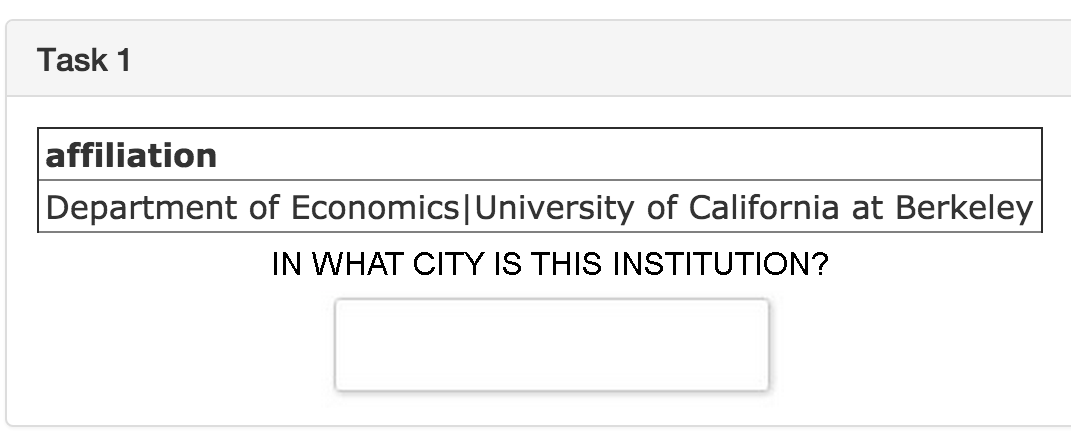
\includegraphics[scale=0.25]{figs/entry.png}
\caption{Example of the Extraction Crowd Interface. \label{fig:entry}}\vspace{-.5em}
\end{figure}

\subsection{Filtering}
We provide an interface for a user defined predicate.
However, as with extraction, filtering has many opportunities for crowdsourcing.
For a filtering operation, the crowd response is binary in contrast to Extraction.
We provide crowd templates for two types of filtering tasks.

\noindent\textbf{Condition Checking: } Given a single record, a crowd worker indicates if it satisfies some condition. In Figure \ref{fig:condition},
we illustrate an example condition checking task.
\begin{figure}[ht!]
\centering
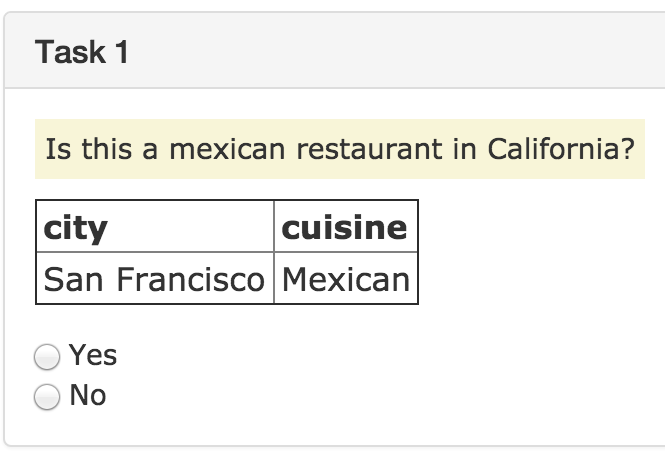
\includegraphics[scale=0.25]{figs/condition.png}
\caption{Condition checking is one variant of the filtering crowd interface.\label{fig:condition}}\vspace{-.5em}
\end{figure}

\noindent\textbf{Pair Comparison: } Given a pair of records, a crowd worker indicates if they are the same or are different. In Figure \ref{fig:pair},
we illustrate an example pair comparison task.

\begin{figure}[ht!]
\centering
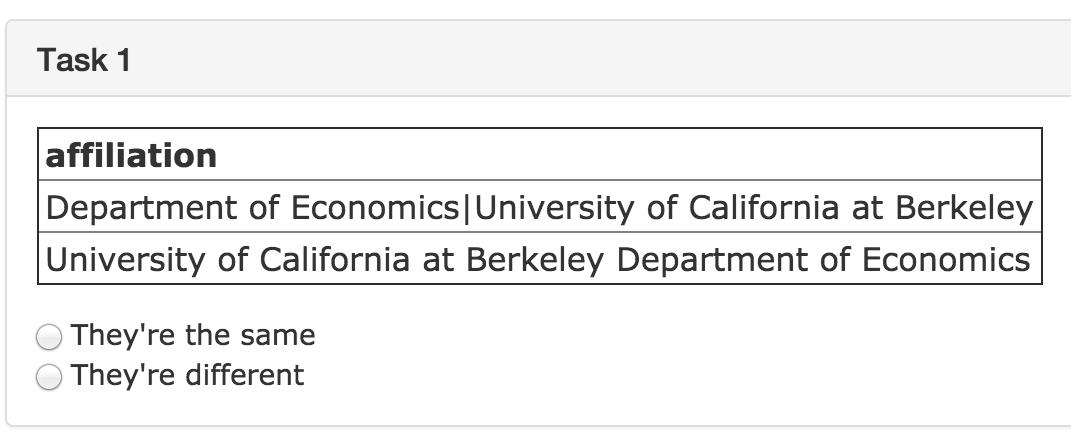
\includegraphics[scale=0.25]{figs/pair.png}
\caption{Pair comparison is the other variant of the filtering crowd interface.\label{fig:pair}}\vspace{-.5em}
\end{figure}

\subsection{Learning Parameters From Example}
In simple cases, it might be easy to use domain knowledge to select and tune physical operators. 
In more complex cases, it might be easier to specify a sample of dirty and clean data instead of the function.
It may also not be feasible to have the crowd clean the entire dataset.
In these cases, we want to learn a statistical model from which we can extrapolate those responses to the rest 
of the data.

In our current implementation of \projx, we pose this learning problem as classification problems.
In general, these parameter functions can be quite complex and this is a simplification of the learning problem.
The choice of classifier and featurization is upto the user. 
We currently support Support Vector Machines and Decision Trees with a featurization library that includes common text processing features.

\vspace{0.5em}

\noindent \textsf{Filter(R, $\mathcal{T}^+$, $\mathcal{T}^-$)}: Given a set of positive training examples $\mathcal{T}^+$ (i.e, $r$ that satisfy the condition) and
negative training examples $\mathcal{T}^-$ (i.e, r that do not satisfy the condition), we learn a classifier that predicts whether a record satisfies the condition. 

\vspace{0.5em}

\noindent \textsf{Extract(R, a, $\mathcal{T}$)} We restrict the learned problem setting to delimited extraction. Given a set of training examples $R(a)$ and the output $v_1,v_2,...,v_k$, we learn a classifier to predict which characters in $R(a)$ are delimiters based on the tokens in the string.

\vspace{1em}

To acquire the samples of clean data, uniform sampling may not be the best strategy.
For example, if there examples of dirty data are very rare, we will not be able to learn a model.
We implement a technique called Active Learning to sample.
Active Learning selects the most informative examples based on the current model so far.
We use an Active Learning algorithm called uncertainty sampling to do this.









%\section{\projx DSL}
We design a DSL for the composition of data cleaning operations.
The general syntax of this language is:
\begin{lstlisting}
<logical operator> on <relations>
	with <physical operators> , <params>
\end{lstlisting}
In this section, we will highlight some key examples.
We have an additional operator \textsf{Async} which designates the 
execution of the operator to be synchronous or asynchronous.

\subsection{String Extraction}
One of the most common data cleaning operations is delimited extraction.
In our DSL, this can be expressed in the following way:
\begin{lstlisting}
Extract on Data
with Split, `,',
cols=[col1, col2]
\end{lstlisting}

We can also use a format string:
\begin{lstlisting}
Extract on Data
with FmtString, `%s:%s',
cols=[col1, col2]
\end{lstlisting}

\subsection{Crowd Entity Resolution}
Crowd-based techniques for entity resolution are increasingly popular e.g Corleone \cite{DBLP:conf/sigmod/GokhaleDDNRSZ14}.
We present an example of expressing a crowd-based technique for entity resolution with the DSL.
Let us suppose we have a database of addresses that we want to deduplicat.
The first step is to group similar rows together and a good similarity metric to use is JaccardSimilarity.
\begin{lstlisting}
SimilarityJoin on Data
with Jaccard, thresh=0.8
\end{lstlisting}
The next step is to filter these pairs using the crowd. 
However, since most pairs will not be duplicates we want to use Active Learning.
Furthermore, since the crowd might be slow, we can add asynchrony.
\begin{lstlisting}
Filter on
( 
 SimilarityJoin on Data
 with Jaccard, thresh=0.8
)
with Crowd, Active, Async
\end{lstlisting}
To resolve the changes, we apply transitive closure at the end that takes the 
longest address:
\begin{lstlisting}
TransitiveClosure (
 Filter on
 ( 
  SimilarityJoin on Data
  with Jaccard, thresh=0.8
 )
 with Crowd, Active
) with Longest
\end{lstlisting}




% !TEX root = demo.tex
\section{Demonstration}
In this section, we detail the proposed demonstration.
The objective of this demonstration is to illustrate 
how \sys enables the rapid iterative construction of data cleaning plans
and the ability to transfer workflows between similar dirty datasets.

\subsection{Datasets}
In our demo, we will consider entity resolution tasks on two different restaurant datasets.
The first dataset contains 858 Zagat reviews\footnote{\scriptsize{ \url{www.cs.utexas.edu/users/ml/riddle/data/restaurant.tar.gz}}},
each tagged with the cuisine of the restaurant reviewed (e.g. ``Chinese" or ``French").
The second dataset is from Yelp and contains 58,127 restaurant records that are also tagged with a category.
In both datasets, tags are inconsistent across records, e.g. ``Chinese" vs. ``Chinese Cuisine".
We will use \sys to merge similar categories together and find the top 10 most popular categories in the dataset.

\begin{figure}[t]
\centering
 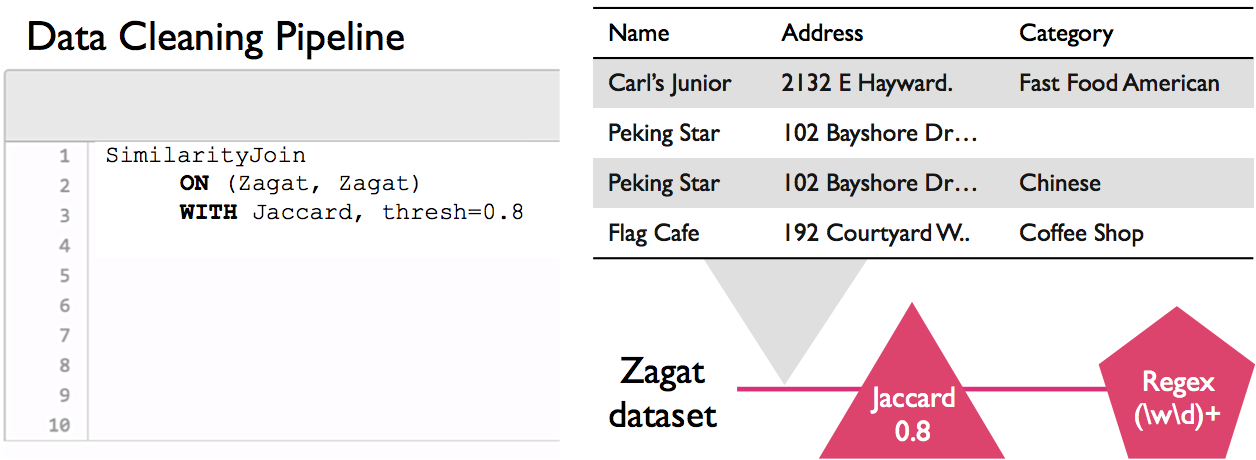
\includegraphics[width=\columnwidth]{figs/dashboard_screenshot.png}
 \caption{The dashboard contains both a visual interface and a text box to specify data cleaning operations. When the user is satisfied, she can run the plan and see the results on the right. \label{screenshot}}
\end{figure}


\begin{figure}[t]
\centering
 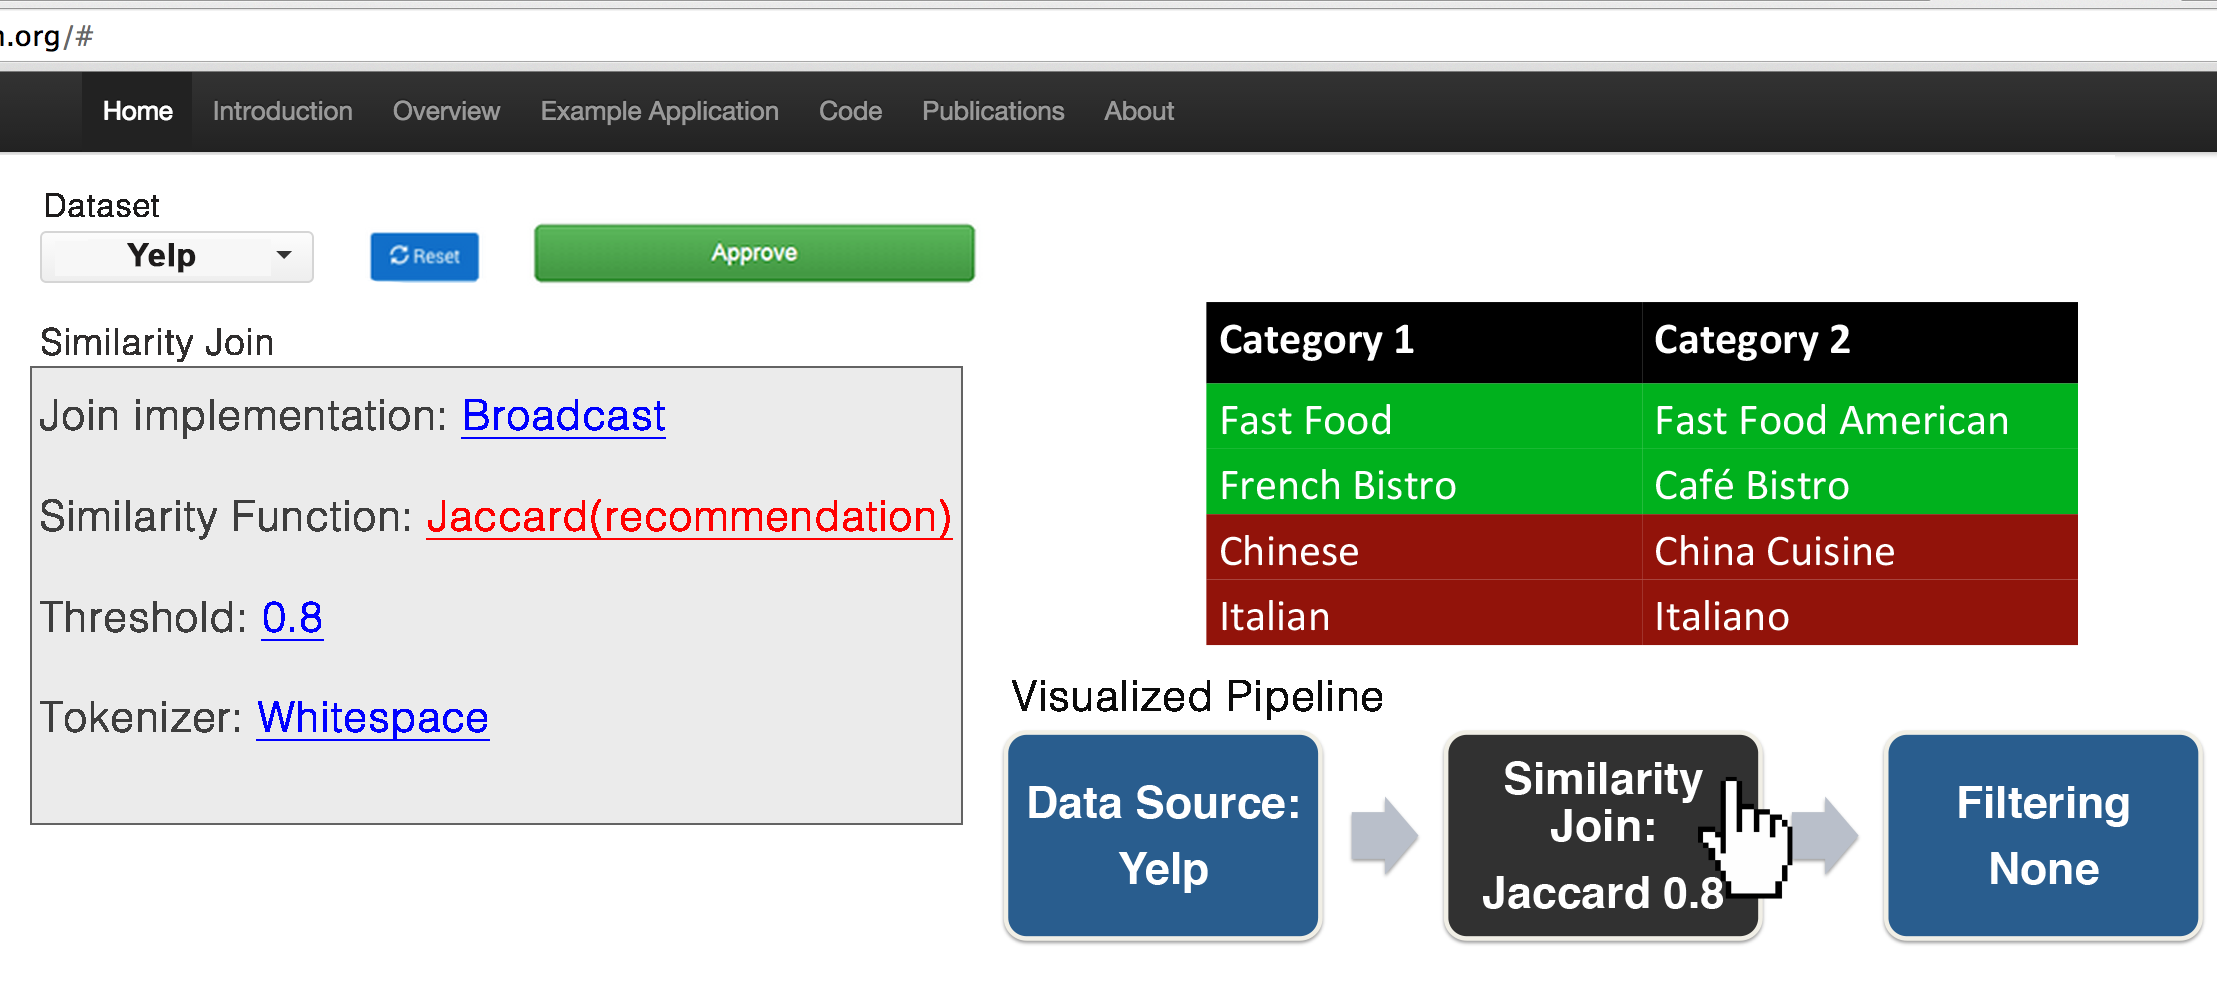
\includegraphics[width=\columnwidth]{figs/dashboard_recsys.png}
 \caption{The operator view lists the parameters of an operator. Users can view recommended changes and modify parameters on the fly.}
 \label{screenshot-rec}\vspace{-1.75em}
\end{figure}

\subsection{Demo Walkthrough}
Now, we will detail the steps of the proposed demonstration.
A screenshot of our dashboard interface is illustrated in Figure \ref{screenshot}.

\vspace{0.2em}

\noindent\textbf{Step 1: } We will explain the components of our dashboard interface to the
demo participants, including how to design data cleaning plans with the visual 
drop down menus, how to compile those plans to our DSL, and how to evaluate the results.

\vspace{0.2em}

\noindent\textbf{Step 2: } Our dashboard will be pre-populated with a data cleaning plan for tag deduplication, and will
start off with the Zagat restaurant dataset. Participants will have the option of choosing one of two Similarity Join implementations, Edit Distance and Jaccard Similarity, and can tune the thresholds for either.
Participants can also add a crowdsourced filtering step in addition to similarity thresholding. 

\vspace{0.2em}

\noindent\textbf{Step 3: } When a participant is satisfied with a plan, they can hit ``Approve" to execute the data cleaning. 
If they chose to use crowdsourcing, then they can complete crowd tasks. 
The results of the plan are visualized in the upper right of our interface.
We show a representative sample of changed records allowing the participant to understand how cleaning affects the data. 
Participants can further analyze their plan by clicking on an operator (Figure \ref{screenshot-rec}).
In addition to the parameters, this shows the recommended changes to the operator.
For example, Figure \ref{screenshot-rec}, shows a recommendation to change the similarity metric from Jaccard to Edit Distance since the attribute in question does not have many tokens.

\vspace{0.2em}

\noindent\textbf{Step 4: } Participants can then switch datasets and observe how the same plan performs on another dataset.
They can modify the plan using the visual interface until the results are satisfactory.

%\section{Conclusion}
In this demonstration, we present a prototype of our \projx system.
Our demonstration concludes with the following take-away messages:
(1) It is beneficial to have an integrated data cleaning solution in the analytics stack,
(2) \projx is a general purpose system that implements many of the salient features of sample-and-clean and progressive data cleaning frameworks, and
(3) the API is concise and intuitive to use.

\section{Acknowledgments}
This research is supported in part by NSF CISE Expeditions award CCF-1139158 and DARPA XData Award FA8750-12-2-0331, and  gifts from Amazon Web Services, Google, SAP,  Apple, Inc., Cisco, Clearstory Data, Cloudera, Ericsson, Facebook, GameOnTalis, General Electric, Hortonworks, Huawei, Intel, Microsoft, NetApp, Oracle, Samsung, Splunk, VMware, WANdisco and Yahoo!.













{
\bibliographystyle{abbrv}
\fontsize{7pt}{7.9pt} \selectfont
\bibliography{refs/bigdata}
}



\end{document}
